\subsection{Hamilton-Operator}
Der allgemeine Hamilton\-/Operator für Moleküle mit $N$ Elektronen und $M$ Atomkernen lautet:
\begin{flalign}\label{hamilton}
  \hat{H} &= -\sum_i^N \frac{1}{2} \nabla_i^2 
            -\sum_A^M \frac{1}{2 m_A} \nabla_A^2
            -\sum_i^N \sum_A^M \frac{Z_A}{r_{iA}}
            +\frac{1}{2}\sum_{i\neq j} \frac{1}{r_{ij}}
            +\frac{1}{2}\sum_{A \neq B } \frac{Z_A Z_B}{r_{AB}}\nonumber\\
          &= \hat{T}_e + \hat{T}_a + \hat{V}_{ea} + \hat{V}_{ee} + \hat{V}_{aa}
\end{flalign}
Dabei steht $Z_A$ für die Ladung des Atomkerns $A$ und 
$r$ für den Abstand zwischen Elektronen und/oder Atomkernen.

\cite[S. 6]{tc2_1}

Die einzelnen Terme haben folgende Bedeutungen:
\begin{enumerate}
    \item $\hat{T}_e$,
    die kinetische Energie aller Elektronen.
    \item $\hat{T}_a$,
    die kinetische Energie aller Atomkerne.
    \item $\hat{V}_{ea}$,
    die potenzielle Energie zwischen allen Elektronen und Atomkernen.
    \item $\hat{V}_{ee}$,
    die potenzielle Energie zwischen allen Elektronen untereinander.
    \item $\hat{V}_{aa}$,
    die potenzielle Energie zwischen allen Atomkernen untereinander.
\end{enumerate}

\subsection{Born-Oppenheimer-Näherung}
Aufgrund des hohen Massenunterschieds zwischen Elektronen und Atomkernen
ist der Einfluss der Elektronen auf die Bewegung der trägeren Atomkerne vernachlässigbar.
Deshalb können bei der Berechnung der Elektronen\-/Wellenfunktion 
die Atomkerne approximativ als statisch betrachtet werden.

Dafür wird der allgemeine Hamilton-Operator \cref{hamilton} aufgeteilt:
\begin{flalign}
  \hat{H} &= \hat{T}_e + \hat{T}_a + \hat{V}_{ea} + \hat{V}_{ee} + \hat{V}_{aa} \nonumber\\
          &= \hat{T}_a + \hat{V}_{aa} + \hat{H}_{\text{el}} \nonumber\\
  \hat{H}_{\text{el}} &= \hat{T}_e + \hat{V}_{ea} + \hat{V}_{ee}
\end{flalign}
Wir lösen nun die Schrödingergleichung \cref*{schroedinger}
mit dem elektronischen Hamilton-Operator $\hat{H}_{\text{el}}$.
Bei der Lösung dieser wird eine feste Kerngeometrie angenommen, 
die wir bei dem Operator $\hat{V}_{eA}$ verwenden werden. 
Mit der resultierenden Elektronen\-/Wellenfunktionen 
lässt sich dann eine Gesamte Wellenfunktion unter Einbezug der Atomkerne konstruieren.

\cite[S. 11-14]{tc2_1}

\subsection{Variationsformulierung}
Da eine analytische Lösung zur Schrödingergleichung nur in speziellen Fällen existiert
\cite[S. 195]{lewars_2016},
wird die exakte Wellenfunktion durch eine Test\-/Wellenfunktion approximiert.
Es lässt sich zeigen, 
dass die Energie dieser Test\-/Wellenfunktion $E_{test}$ 
immer über der tatsächlichen Energie $E_0$ liegt.

\subsubsection*{Beweis}
Voraussetzungen:
\begin{enumerate}
  \item Der Hamiltonian $\hat{H}$ hat die Eigenfunktionen $\psi_i^{}$ mit Eigenwerten $E_i^{}$.
  \item Es existiert eine Eigenfunktion $\psi_0^{}$ mit dem niedrigsten  Eigenwert $E_0^{}$.
  \item Alle Eigenfunktion von $\hat{H}$ sind orthonomal zueinander:\\
  $\langle \psi_i^{} \vert \psi_j^{} \rangle = \delta_{ij}^{},\quad\forall i,j$
  \item Die Test-Wellenfunktion lässt sich als Linearkombination der Eigenfunktionen darstellen:
  $\psi_{test}^{} = \sum_{n}^{} c_n^{} \psi_n^{}$
\end{enumerate}

Die Voraussetzungen (1), (3) und (4) sind anzunehmen, da der Hamiltonian hermitesch ist.
Die 2. Voraussetzung hingegen entspricht unserer physikalischen Realität.

Es ist zu zeigen: $E_{test}^{} \geq E_0^{}$ oder $E_{test}^{} - E_0^{} \geq 0$
\begin{flalign*}
  E_{test} - E_0 
  &= \langle \psi_{test}^{} \vert \hat{H} - E_0^{} \vert \psi_{test}^{} \rangle\\
  &= \int \psi_{test}^* (\hat{H} - E_0^{}) \psi_{test}^{} \,dx \quad &\vert \text{ 4. Voraussetzung}\\
  &= \sum_n \sum_m c_n^\ast c_m^{} \int \psi_{n}^* (\hat{H} - E_0^{}) \psi_{m} \,dx 
  \quad &\vert \text{ 1. Voraussetzung}\\
  &= \sum_n \sum_m c_n^\ast c_m^{} \int \psi_{n}^* (E_m^{} - E_0^{}) \psi_{m} \,dx 
  \quad &\vert \text{ 3. Voraussetzung}\\
  &= \sum_n \left\lvert c_n^{} \right\rvert^2 (E_n^{} - E_0^{}) \int \psi_{n}^* \psi_{n} \,dx 
  \quad &\vert \text{ 3. Voraussetzung}\\
  &= \sum_n \left\lvert c_n^{} \right\rvert^2 (E_n^{} - E_0^{})
  \quad &\vert \text{ 2. Voraussetzung}\\
  &\geq 0 &\qed
\end{flalign*}
\cite[S. 187]{atkins_friedman_2011}

\subsection{Beschreibung von Elektronen}\label{section_slater}
Die Form der Wellenfunktion für Elektronen ist in diesem Modell nicht nur 
durch die Schrödingergleichung \cref{schroedinger} gegeben.
Um ein realitätsnahes Bild von Elektronen zu schaffen,
muss die Wellenfunktionen zusätliche Forderungen erfüllen.
Diese unerfassten Eigenschaften sind das intrinsisches Drehmoment des Elektrons,
auch Spin genannt, und die Antisymmetrie der Wellenfunktion
im Bezug auf den Austausch zweier Elektronen.
Wir stellen diese zusätzlichen Forderungen,
weil diese Eigenschaften experimentell beobachtbar sind.
Anzumerken ist, dass diese Bedingungen an die Wellenfunktion 
in einer relativistischen Behandlung von selbst entstehen
und nicht wie hier künstlich eingebaut werden müssen.

\cite[S. 265, 270]{levine_2019}
\cite[4.5.3]{cramer_2004}

\subsubsection*{Notation}
Da jedes Elektron mindestens 3 Parameter ($x, y, z$) zur Beschreibung benötigt,
kann dies bei größeren Systemen schnell unübersichtlich werden.
Deshalb ist es üblich die Parameter eines Elektrons durch eine natürliche Zahl abzukürzen:

\begin{equation}
    \Psi(1, 2, 3, \dots) \equiv  \Psi(x_1, y_1, z_1, \quad
    x_2, y_2, z_2,\quad x_3, y_3, z_3, \quad\dots)
\end{equation}

Diese verkürzte Notation wird in der restlichen Arbeit verwendet.

\subsubsection*{1. Spin}\label{spin-section}
Jedes Elektron verfügt, neben einer räumlichen Ausdehnung, 
auch über einen intrinsischen Spin. 
Ein Elektron kann lediglich zwei Spin\-/Zustände annehmen.
Diese Zustände werden mit den Spinfunktionen $\alpha$ und
$\beta$ dargestellt und sind gegeben durch:
\begin{equation}\label{spin_function}
  \begin{aligned}
    \alpha(\omega) &:= \delta(\omega - \nicefrac{1}{2})\\
    \beta(\omega) &:= \delta(\omega + \nicefrac{1}{2})
  \end{aligned}
\end{equation}
mit den Eigenschaften:
\begin{equation}\label{spin_product}
  \begin{aligned}
    \langle \alpha \vert \alpha \rangle &= \langle \beta \vert \beta \rangle = 1 \\
    \langle \alpha \vert \beta \rangle &= \langle \beta \vert \alpha \rangle = 0
  \end{aligned}
\end{equation}

Die Spinkoordinate $\omega$ existiert separat von den räumlichen Koordinaten $x,y,z$.
Deshalb hängt die Wellenfunktion $\varphi$ eines einzigen Elektrons
von insgesamt vier Parametern ab
und wird als Produkt einer Raum- und Spin\-/Funktion dargestellt.
Im Kontext eines Moleküls werden die Raumwellenfunktionen auch Orbitale genannt, welche
je zwei Elektronen mit entgegengesetztem Spin enthalten können.
Das Produkt der Raum- und Spin\-/Funktion wird deshalb auch als Spinorbital bezeichnet.

\begin{equation}\label{spin}
  \varphi(1) := \varphi(x_1, y_1, z_1, \omega_1) = \begin{cases}
    \psi(x_1, y_1, z_1) \alpha(\omega_1) = \psi(1) \alpha(1)\\
    \psi(x_1, y_1, z_1) \beta(\omega_1) = \psi(1) \beta(1)\\
  \end{cases}
\end{equation}

Zu beachten ist, dass Elektronen nur für die Werte 
$\omega = \pm \nicefrac{1}{2}$ existieren können ($\lvert \varphi \rvert^2 > 0$) und
der Parametersatz eines Elektrons durch eine natürliche Zahl abgekürzt werden kann.

\cite[S. 45]{szabo_ostlund_1996}

Diese Spin-Eigenschaft wurde erstmals im Stern-Gerlach-Experiment (1921) beobachtet, 
welches in Frankfurt am Main durchgeführt wurde.
\cite{tc1_spin}

\begin{figure}[h]
\begin{center}
    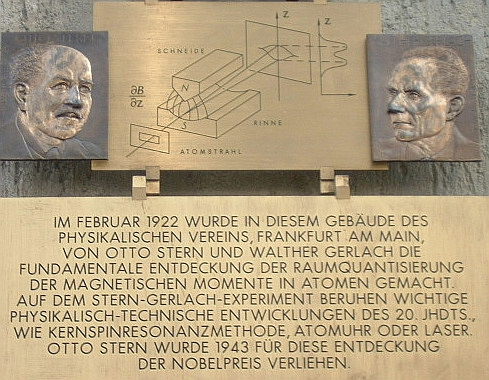
\includegraphics[width=0.75\textwidth]{res/sterngerlach2.jpg}
\end{center}
    \caption{Plakette zum Gedenken an das Stern-Gerlach-Experiment. \cite{sterngerlach}}
\end{figure}


\subsubsection*{2. Antisymmetrie}
Diese Forderung besagt, dass eine Elektronen\-/Wellenfunktion im Bezug auf
den Austausch zweier beliebiger Elektronen\-/Koordinaten antisymmetrisch sein muss:

\begin{equation}\label{antisymmetry}
  \Psi(1, \dots, i, \dots, j, \dots, N) = - \Psi(1, \dots, j, \dots, i, \dots, N), \quad \forall i,j
\end{equation}

\cite[S. 45, 46]{szabo_ostlund_1996}

\subsubsection*{Pauli-Ausschluss-Prinzip}
Aus \cref{spin_product}, \cref{spin} und \cref{antisymmetry} folgt,
dass zwei Elektronen mit identischem Spin sich nicht an
den gleichen Raumkoordinaten aufhalten können. Dies ergibt sich aus folgendem Beweis:

Nehmen wir an, dass zwei Elektronen $i,j$ die selben Raum- und Spin\-/Koordinaten ($i = j$) haben:
\begin{equation*}
  \Psi(1, \dots, i, \dots, j, \dots, N) = \Psi(1, \dots, i, \dots, i, \dots, N)
\end{equation*}
Wir fordern auch Antisymmetrie:
\begin{equation*}
  \Psi(1, \dots, i, \dots, j, \dots, N) = -\Psi(1, \dots, j, \dots, i, \dots, N)
\end{equation*}
Es folgt daher:
\begin{flalign*}
  \Psi(1, \dots, i, \dots, i, \dots, N) &= -\Psi(1, \dots, i, \dots, i, \dots, N) \\
  2\Psi(1, \dots, i, \dots, i, \dots, N) &= 0
\end{flalign*}
$\Rightarrow$ Die Wahrscheinlichkeit, dass zwei Elektronen mit gleichem Spin 
sich am selben Ort befinden ist null. \qed

Dieses Phänomen auf Spinorbitalen angewandt bedeutet,
dass zwei Elektronen nicht das selbe Spinorbital besetzen können,
dies nennt man das Pauli\-/Ausschluss\-/Prinzip.
Das resultierende Meiden der Elektronen wird Pauli\-/Repulsion genannt.

\cite[S. 271, 276]{levine_2019}

\subsubsection*{Slater-Determinante}
Um sowohl Spin als auch die Antisymmetrie in unsere Wellenfunktion einzubinden,
wird diese als Determinante von Spinorbitalen ausgedrückt.
Dabei wird pro Elektron ein Spinorbital verwendet.

\begin{equation}\label{slater}
\Psi(1, \dots, N) = 
\frac{1}{\sqrt{N!}}
\left\lvert
\begin{array}{ccccc} 
\varphi_1(1)  & \varphi_2(1)  & \cdots & \varphi_{N-1}(1)  & \varphi_N(1)\\ 
\varphi_1(2)  & \varphi_2(2)  & \cdots & \varphi_{N-1}(2)  & \varphi_N(2)\\ 
\vdots        & \vdots        & \ddots & \vdots            & \vdots      \\ 
\varphi_1(N)  & \varphi_2(N)  & \cdots & \varphi_{N-1}(N)  & \varphi_N(N)
\end{array}
\right\rvert
\end{equation}

Vertauschen wir zwei Elektronen, gleicht das einem Tausch zweier Zeilen
und das Vorzeichen der Determinante ändert sich.
Die Antisymmetrie unserer Wellenfunktion ist gegeben.

Sollten zwei Elektronen das selbe Spinorbital besetzen,
so wären zwei Spalten identisch, wodurch die Determinante verschwindet.
Das Pauli\-/Ausschluss\-/Prinzip ist ebenfalls erfüllt.

\cite[S. 50]{szabo_ostlund_1996}

Sollte jedes Raumorbital doppelt besetzt sein,
so können wir $\Psi$ mit nur $n$ Raumorbitalen ($2n = N$) darstellen:
\begin{equation}
\Psi(1, \dots, 2n) = 
\frac{1}{\sqrt{(2n)!}}
\left\lvert
\begin{array}{ccccc} 
\psi_1(1)\alpha(1) & \psi_1(1)\beta(1) & \cdots & \psi_n(1)\alpha(1) & \psi_n(1)\beta(1)\\ 
\psi_1(2)\alpha(2) & \psi_1(2)\beta(2) & \cdots & \psi_n(2)\alpha(2) & \psi_n(2)\beta(2)\\ 
    \vdots         &       \vdots      & \ddots &       \vdots       &       \vdots     \\ 
\psi_1(2n)\alpha(2n) & \psi_1(2n)\beta(2n) & \cdots & \psi_n(2n)\alpha(2n) & \psi_n(2n) \beta(2n)
\end{array}
\right\rvert
\end{equation}
\cite[S. 202]{lewars_2016}

Wir haben nun eine Beschreibung für die Elektronen\-/Wellenfunktion erhalten,
die in der Hartree\-/Fock\-/Theorie verwendet wird.

Um die Theorie überschaubar zu halten,
werden nur Molekulare\-/Systeme mit doppelt besetzten Raumorbitalen betrachtet.